% ============================================================
% v4 演示波④ · 滚动小卷（一）（范围 1.1：§1.1.1＋§1.1.2＋§1.1.3 跨节混编）
% 件型依据：拍板19（滚动小卷：跨节混编范围小卷、45分钟100分、单选6＋多选2…、
%   抽题纯编排不新命制、件型名自拟守§6）＋总诊断§三。
% 版式＝样张v4/测评卷 横放3栏惯用法拷贝改造：A4 横放 3 栏（栏宽≈84mm、栏距 8mm、无栏线）；
%   卷头瘦身 ≤30mm 占首栏、卷名 16pt、卷头标「45分钟 100分」；撤页眉；页脚单行 DDDDDD
%   灰块页码离底 ≈11mm；分区标题同号连排；题间距 3pt；题号悬挂 7mm；选项 4/2/1 网格
%   （分号字符全保留）；题侧挂难度＋（知识点N）＋★（6.5pt #777777 内联防折行；跨节题
%   标原节知识点号，映射见交付报告台账）；解答题分值题号后（全品位）；不留作答留白；
%   \linespread{1}＋\raggedcolumns；纯灰阶 黑＋777777＋DDDDDD。
% 题源：讲练件（上）§1.1.1 题型组 5 题（≡v3测评卷源池，拍板37 口径逐对登记）＋
%   §1.1.2 3 题＋§1.1.3 6 题（均未入三件套）。逐题台账见交付报告.md。
% 配分（全品滚动习题(一) p16–p17 实证口径）：单选6×5＋多选2×6＋填空3×5＋解答3题
%   （13＋15＋15）＝100分，共14题。
% 编译：xelatex main.tex（两遍）→ render.py（先清 png/）→ 断言题号列.py＋断言版式.py
% ============================================================
\documentclass[fontset=none]{ctexart}

% ---------- 字体（同测评卷 v4） ----------
\setmainfont{Times New Roman}
\setCJKmainfont[BoldFont=SimHei]{SimSun}
\setCJKfamilyfont{hei}{SimHei}
\newcommand{\heiti}{\CJKfamily{hei}}
\xeCJKDeclareCharClass{CJK}{"2460->"24FF, "2200->"22FF, "25A0->"25FF, "2600->"26FF}
\xeCJKsetup{CheckSingle=true}

% ---------- 宏包 ----------
\usepackage[a4paper,landscape,top=15mm,bottom=17.33mm,left=15mm,right=15mm,headheight=12pt,headsep=2mm,footskip=3mm]{geometry}
\usepackage{amsmath,amssymb}
\usepackage{graphicx}
\usepackage{xcolor}
\usepackage{multirow,array,calc}
\usepackage{multicol}
\usepackage{needspace}
\usepackage{fancyhdr}
\usepackage{indentfirst}
\usepackage{tikz}

% ---------- 颜色（纯灰阶：黑＋777777＋DDDDDD） ----------
\definecolor{pnumbg}{HTML}{DDDDDD}
\definecolor{kygray}{HTML}{777777}

% ---------- 版面（横放 3 栏，同测评卷 v4） ----------
\linespread{1}
\renewcommand{\normalsize}{\fontsize{10.5pt}{18pt}\selectfont}
\normalsize
\setlength{\columnsep}{8mm}
\setlength{\columnseprule}{0pt}
\setlength{\multicolsep}{0pt}
\setlength{\parindent}{2em}
\clubpenalty=10000
\widowpenalty=10000
\displaywidowpenalty=10000
\tolerance=9999
\binoppenalty=100
\relpenalty=100
\raggedbottom

\setlength{\arrayrulewidth}{0.4pt}
\setlength{\tabcolsep}{3pt}
\renewcommand{\arraystretch}{1.3}

% ---------- 页脚（单行灰块页码，底缘离页底≈11mm，同测评卷 v4） ----------
\newcommand{\footblock}{{\setlength{\fboxsep}{0pt}\colorbox{pnumbg}{%
  \makebox[31mm][c]{\rule[-1.45mm]{0pt}{5mm}\fontsize{10.5pt}{12pt}\selectfont\bfseries\thepage}}}}
\pagestyle{fancy}
\fancyhf{}
\fancyfoot[C]{\footblock}
\renewcommand{\headrulewidth}{0pt}

% ---------- 自定义命令（同测评卷 v4） ----------
\newcommand{\glueguard}[1]{\vskip 0pt plus #1\baselineskip\penalty-100\vskip 0pt plus -#1\baselineskip}
\newcommand{\sidemark}[3]{{\fontsize{6.5pt}{8pt}\selectfont\color{kygray}#1#2（知识点#3）}}
\newcommand{\fenzhi}[1]{{\mdseries（#1分）}}
\newcommand{\timu}[5]{\par\glueguard{4}\addvspace{3pt}%
  \noindent\hangindent=7mm\hangafter=1\textbf{#1}\sidemark{#2}{#3}{#4}\,#5\par}
\newcommand{\quku}[2]{\par\glueguard{6}\addvspace{2pt}%
  \noindent{\heiti #1}#2\par\addvspace{1pt}}
\newcommand{\biaoqian}[1]{{\heiti #1}}
\newcommand{\kongbai}{\underline{\hspace*{15mm}}}
\newcommand{\juanline}{\underline{\hspace*{12mm}}}
\newcommand{\ansval}[1]{\underline{#1}}
\newcommand{\daan}[3]{\par\glueguard{3}\addvspace{5pt}%
  \noindent\hangindent=7mm\hangafter=1\textbf{#1}\ansval{#2}\quad #3\par}
\newcommand{\opts}[1]{\par\penalty10000\noindent\hangindent=7mm\hangafter=0#1\par\penalty10000}
\newcommand{\figblk}[1]{\penalty10000\noindent\hangindent=0pt\hangafter=1\hspace*{7mm}%
  \makebox[\dimexpr\linewidth-7mm\relax][c]{\includegraphics[width=30mm]{#1}}\par\penalty10000}

\begin{document}

\begin{multicols}{3}
\raggedcolumns
\emergencystretch=8em

% ================= 卷头（瘦身 ≤30mm、占首栏；全品滚动习题 p16 口径） =================
{\centering
{\fontsize{10.5pt}{13.3pt}\selectfont 班级：\juanline\quad 姓名：\juanline\quad 考号：\juanline\par}
\vspace{1pt}
{\fontsize{16pt}{18pt}\selectfont\heiti 滚动小卷（一）\par
\vspace{1pt}·\ 范围 1.1\par}
\vspace{1pt}
{\fontsize{10.5pt}{13.3pt}\selectfont （时间：45分钟\quad 满分：100分）\par}
\vspace{1pt}
{\fontsize{10.5pt}{13.3pt}\selectfont 考生注意：请在答题纸上作答，答在本卷上无效。\par}
}
\vspace{2pt}

% ================= 一、单项选择题（6×5＝30分） =================
\quku{一、单项选择题（每小题5分，共30分）}{本大题共6小题，在每小题给出的四个选项中，只有一项是符合题目要求的。}

\timu{1．}{简单}{}{1}{下列说法正确的是（~~~~）}

\opts{A．若\(\left| \overrightarrow{a} \right| = \allowbreak\left| \overrightarrow{b} \right|\)，则\(\overrightarrow{a} = \overrightarrow{b}\)或\(\overrightarrow{a} = - \overrightarrow{b}\)；\newline B．若\(\overrightarrow{a},\overrightarrow{b}\)为相反向量，则\(\overrightarrow{a} + \overrightarrow{b} = \overrightarrow{0}\)；\newline C．零向量是没有方向的向量；\newline D．若\(\overrightarrow{a},\overrightarrow{b}\)是两个单位向量，则\(\overrightarrow{a} = \overrightarrow{b}\)}

\timu{2．}{简单}{}{1}{若\(\{ \overrightarrow{a},\overrightarrow{b},\overrightarrow{c} \}\)是空间的一个基底，则下列各组中不能构成空间的一个基底的是（~~~~）.}

\opts{A．\(\overrightarrow{a}\)，\(2\overrightarrow{b}\)，\(3\overrightarrow{c}\)；B．\(\overrightarrow{a}+\overrightarrow{b}\)，\(\overrightarrow{b}+\overrightarrow{c}\)，\(\overrightarrow{c}+\overrightarrow{a}\)；\newline C．\(\overrightarrow{a}+\overrightarrow{b}+\overrightarrow{c}\)，\(\overrightarrow{b}+\overrightarrow{c}\)，\(\overrightarrow{c}\)；D．\(\overrightarrow{a}+2\overrightarrow{b}\)，\(2\overrightarrow{b}+3\overrightarrow{c}\)，\(3\overrightarrow{a}-9\overrightarrow{c}\)}

\timu{3．}{简单}{}{4}{已知\(A(1,2,-1)\)关于面\(xOy\)的对称点为\(B\)，而\(B\)关于\(x\)轴的对称点为\(C\)，则\(\overrightarrow{BC}\)等于（~~~~）}

\opts{A．\((0,4,2)\)；B．\((-2,0,0)\)；\newline C．\((0,-4,-2)\)；D．\((2,0,-2)\)}

\timu{4．}{简单}{}{7}{在空间直角坐标系中，已知\(M(-1,0,2)\)，\(N(3,2,-4)\)，则\(MN\)的中点\(P\)到坐标原点\(O\)的距离为（~~~~）}

\opts{A．\(\sqrt{3}\)；B．\(\sqrt{2}\)；C．2；D．3}

\timu{5．}{中档}{}{6}{在棱长为1的正方体\(ABCD - A_{1}B_{1}C_{1}D_{1}\)中，\(P\)是底面\(ABCD\)上（含边界）一动点，满足\(A_{1}P \perp AC_{1}\)，则线段\(A_{1}P\)长度的取值范围（~~~~）}

\opts{A．\(\left[ \frac{\sqrt{6}}{2},\sqrt{2} \right]\)；B．\(\left[ \frac{\sqrt{6}}{2},\sqrt{3} \right]\)；\newline C．\(\lbrack 1,\sqrt{2}\rbrack\)；D．\(\left[ \sqrt{2},\sqrt{3} \right]\)}

\timu{6．}{中档}{}{3}{如图，在大小为45°的二面角A\-EF\-D中，四边形ABFE，CDEF都是边长为1的正方形，则B，D两点间的距离是()}

\figblk{media/image4.png}

\opts{A．\(\sqrt{3}\)；B．\(\sqrt{2}\)；C．1；D．\(\sqrt{3 - \sqrt{2}}\)}

% ================= 二、多项选择题（2×6＝12分） =================
\quku{二、多项选择题（每小题6分，共12分）}{本大题共2小题，在每小题给出的选项中，有多项符合题目要求。全部选对的得6分，部分选对的得部分分，有选错的得0分。}

\timu{7．}{简单}{★}{3}{设\(\overrightarrow{a}\)，\(\overrightarrow{b}\)为空间中的任意两个非零向量，下列各式中正确的有（~~~~）}

\opts{A．\({\overrightarrow{a}}^{2} = \allowbreak\left| \overrightarrow{a} \right|^{2}\)；\newline B．\(\frac{\overrightarrow{a} \cdot \overrightarrow{b}}{\overrightarrow{a} \cdot \overrightarrow{a}} = \frac{\overrightarrow{b}}{\overrightarrow{a}}\)；\newline C．\(\left( \overrightarrow{a} \cdot \overrightarrow{b} \right)^{2} = {\overrightarrow{a}}^{2} \cdot {\overrightarrow{b}}^{2}\)；\newline D．\(\left( \overrightarrow{a} - \overrightarrow{b} \right)^{2} = {\overrightarrow{a}}^{2} - 2\overrightarrow{a} \cdot \overrightarrow{b} + {\overrightarrow{b}}^{2}\)}

\timu{8．}{简单}{★}{1}{对空间任意一点\(O\)和不共线三点\(A\)，\(B\)，\(C\)，能得到\(P\)，\(A\)，\(B\)，\(C\)四点共面的是（~~~~）}

\opts{A．\(\overrightarrow{OP} = \overrightarrow{OA} + \overrightarrow{OB} + \overrightarrow{OC}\)；\newline B．\(\overrightarrow{OP} = \frac{1}{3}\overrightarrow{OA} + \frac{1}{3}\overrightarrow{OB} + \frac{1}{3}\overrightarrow{OC}\)；\newline C．\(\overrightarrow{OP} = \frac{3}{4}\overrightarrow{OA} + \frac{1}{8}\overrightarrow{OB} + \frac{1}{8}\overrightarrow{OC}\)；\newline D．\(\overrightarrow{OP} = 2\overrightarrow{OA} - \overrightarrow{OB} - \overrightarrow{OC}\)}

% ================= 三、填空题（3×5＝15分） =================
\quku{三、填空题（每小题5分，共15分）}{本大题共3小题。}

\timu{9．}{简单}{}{2}{在直三棱柱\(ABC - A_{1}B_{1}C_{1}\)中，若\(\overrightarrow{CA} = \overrightarrow{a},\overrightarrow{CB} = \overrightarrow{b},\overrightarrow{CC_{1}} = \overrightarrow{c},\)，则\(\overrightarrow{A_{1}B}\)=\kongbai.(用\(\overrightarrow{a},\overrightarrow{b},\overrightarrow{c}\)表示)}

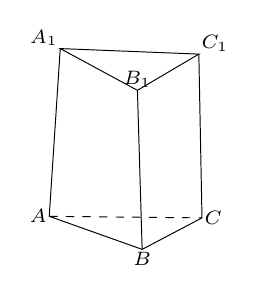
\begin{tikzpicture}[x=1mm,y=1mm,line width=0.35pt,
  every node/.style={font=\fontsize{7.5pt}{8.5pt}\selectfont,inner sep=0.8pt}]
  \coordinate (A1) at (2.2,25.5);
  \coordinate (C1) at (19.8,24.8);
  \coordinate (B1) at (12.0,20.2);
  \coordinate (A)  at (0.8,4.2);
  \coordinate (C)  at (20.2,4.0);
  \coordinate (B)  at (12.6,0);
  \draw (A1) -- (C1) -- (B1) -- cycle;
  \draw (A) -- (B) -- (C);
  \draw[dashed] (A) -- (C);
  \draw (A) -- (A1);
  \draw (B) -- (B1);
  \draw (C) -- (C1);
  \node[above left]  at (A1) {$A_1$};
  \node[above right] at (C1) {$C_1$};
  \node[above]       at (B1) {$B_1$};
  \node[left]        at (A)  {$A$};
  \node[right]       at (C)  {$C$};
  \node[below]       at (B)  {$B$};
\end{tikzpicture}

\timu{10．}{简单}{}{6}{若\(\overrightarrow{a} = (1, - 1,2)\)，向量\(\overrightarrow{AB}\)与\(\overrightarrow{a}\)平行且\(\left| \overrightarrow{AB} \right| = 2\sqrt{6}\)，则\(\overrightarrow{AB} =\)\kongbai.}

\timu{11．}{简单}{}{3}{已知\(\left| \overrightarrow{a} \right| = 3\sqrt{2},\left| \overrightarrow{b} \right| = 4,\)\(\overrightarrow{m} = \overrightarrow{a} + \overrightarrow{b},\overrightarrow{n} = \overrightarrow{a} + \lambda\overrightarrow{b},\left\langle \overrightarrow{a},\overrightarrow{b} \right\rangle = 135{^\circ},\overrightarrow{m}\bot\overrightarrow{n}\) ，则λ＝\kongbai．}

% ================= 四、解答题（3题，13＋15＋15＝43分） =================
\quku{四、解答题（共43分）}{本大题共3小题，解答应写出文字说明、证明过程或演算步骤。}

\timu{12．\fenzhi{13}}{中档}{}{6}{已知向量\(\overrightarrow{a} = (2,4,5)\)，\(\overrightarrow{b} = (3,x,y)\)．}

\opts{(1)若\(\overrightarrow{a}\parallel\overrightarrow{b}\)，求实数\(x\)，\(y\)的值；(2)若\(\overrightarrow{a} \perp \overrightarrow{b}\)，且\(\left| \overrightarrow{b} \right| = \sqrt{29}\)，求实数\(x\)，\(y\)的值．}

\timu{13．\fenzhi{15}}{中档}{★}{1}{如图所示，在平行六面体\(ABCD - A_{1}B_{1}C_{1}D_{1}\)中，\(E\)，\(F\)分别在\(BB_{1}\)和\(DD_{1}\)上，且\(BE = \frac{1}{3}BB_{1}\)，\(DF = \frac{2}{3}DD_{1}\)．}

\figblk{media/gundong_paliujmian.png}

\opts{(1)证明：\(A\)、\(E\)、\(C_{1}\)、\(F\)四点共面．(2)若\(\overrightarrow{EF} = x\overrightarrow{AB} + y\overrightarrow{AD} + z\overrightarrow{AA_{1}}\)，求\(x + y + z\)．}

\timu{14．\fenzhi{15}}{中档}{}{6}{已知点\(A(0,1,2)\)，\(B(1, - 1,3)\)，\(C(1,5, - 1)\)．}

\opts{(1)若\(D\)为线段\(BC\)的中点，求线段\(AD\)的长；(2)若\(\overrightarrow{AD} = (2,a,1)\)，且\(\overrightarrow{AB} \cdot \overrightarrow{AD} = 1\)，求\(a\)的值，并求此时向量\(\overrightarrow{AB}\)与\(\overrightarrow{AD}\)夹角的余弦值．}

\end{multicols}

% ================= 参考答案与解析（另起页，3 栏密集排，同测评卷 v4 惯用法） =================
\clearpage
{\centering
{\fontsize{15pt}{22pt}\selectfont\heiti 参考答案与解析\par}
\vspace{3pt}\noindent\rule{\textwidth}{0.4pt}\par}
\vspace{4pt}

\begin{multicols}{3}
\raggedcolumns
\emergencystretch=8em

\daan{1．}{B}{\biaoqian{【分析】}根据零向量、单位向量、向量的模、相等向量、相反向量等概念逐一分析即可得出答案.\biaoqian{【详解】}解：若\(\left| \overrightarrow{a} \right| = \allowbreak\left| \overrightarrow{b} \right|\)，则它们的方向相同时是相等向量，方向相反时是相反向量，还有可能方向既不相同，也不相反，A错；若\(\overrightarrow{a},\overrightarrow{b}\)为相反向量，则它们的和为零向量，B对；零向量的方向是任意的，C错；两个单位向量只是模都为1，方向不一定相同，D错.故选：B.}

\daan{2．}{D}{\biaoqian{【分析】}由于\(\{ \overrightarrow{a},\overrightarrow{b},\overrightarrow{c} \}\)是空间的一个基底，则可得\(\overrightarrow{a}\)，\(\overrightarrow{b}\)，\(\overrightarrow{c}\)不共面，然后根据空间向量的共面定理，一组不共面的向量构成空间的一个基底，对选项中的向量进行判断即可\biaoqian{【详解】}因为\(\{ \overrightarrow{a},\overrightarrow{b},\overrightarrow{c} \}\)是空间的一个基底，所以\(\overrightarrow{a}\)，\(\overrightarrow{b}\)，\(\overrightarrow{c}\)不共面.
对于A，B，C选项，每组都是不共面的向量，能构成空间的一个基底；
对于D：\(\overrightarrow{a} + 2\overrightarrow{b}\)，\(2\overrightarrow{b} + 3\overrightarrow{c}\)，\(3\overrightarrow{a} - 9\overrightarrow{c}\)满足\(3\overrightarrow{a} - 9\overrightarrow{c} = 3\left[ \left( \overrightarrow{a} + 2\overrightarrow{b} \right) - \left( 2\overrightarrow{b} + 3\overrightarrow{c} \right) \right]\)，所以这三个向量是共面向量，故不能构成空间的一个基底.故选：D.
\biaoqian{【点睛】}此题考查了空间向量共面的判断与应用，属于基础题.}

\daan{3．}{C}{\biaoqian{【分析】}根据空间中点与点的对称性，容易求得\(B,C\)两点的坐标，即可得向量\(\overrightarrow{BC}\).\biaoqian{【详解】}因为\(A(1,2, - 1)\)关于面\(xOy\)的对称点为\(B\)，故\(B(1,2,1)\)；又点\(B\)关于\(x\)轴的对称点为\(C\)，故\(C(1, - 2, - 1)\)，故\(\overrightarrow{BC} = (0, - 4, - 2)\).故选：C.
\biaoqian{【点睛】}本题考查空间中点关于面的对称点的求解，属基础题.}

\daan{4．}{A}{\biaoqian{【分析】}利用中点坐标公式及空间中两点之间的距离公式可得解.\biaoqian{【详解】}\(\because M( - 1,0,2)\)，\(N(3,2, - 4)\)，由中点坐标公式，得\(P(1,1, - 1)\)，所以\(\left| OP \right| = \sqrt{1 + 1 + 1} = \sqrt{3}\).故选：A}

\daan{5．}{A}{\biaoqian{【分析】}利用线面垂直的判定定理可以证明\(AC_{1} \perp\)平面\(BDA_{1}\)，这样可以确定\(P\)的轨迹，利用平面几何的知识求出\(A_{1}P\)的最值，选出答案.\biaoqian{【详解】}因为\(CC_{1} \perp\)底面ABCD，\(DB \subset\)底面ABCD，所以\(CC_{1} \perp BD\)，底面ABCD是正方形，所以有\(CA \perp BD\)，\(CC_{1} \cap CA = C\)，\(CC_{1},CA \subset\)平面\(CC_{1}A\)，因此有\(BD \perp\)平面\(CC_{1}A\)，\(AC_{1} \subset\)平面\(CC_{1}A\)，所以有\(BD \perp AC_{1}\)，同理可证明出\(AC_{1} \perp DA_{1}\)，因为\(BD \cap DA_{1} = D\)，\(BD,DA_{1} \subset\)平面\(BDA_{1}\)，所以\(AC_{1} \perp\)平面\(BDA_{1}\)，所以点\(P\)的轨迹就是线段BD，所以\(P\)在\(B\)或\(D\)时\(A_{1}P\)最长为\(\sqrt{2}\)，在BD中点时\(A_{1}P\)最短为\(\frac{\sqrt{6}}{2}\).故选：A
\biaoqian{【点睛】}本题考查了空间点的轨迹问题，考查了线面垂直的判定定理，考查了推理论证能力.}

\daan{6．}{D}{\biaoqian{【分析】}由\(\overrightarrow{DB} = \overrightarrow{ED} + \overrightarrow{FE} + \overrightarrow{BF}\)，利用数量积运算性质展开即可得到答案\biaoqian{【详解】}\(\because\overrightarrow{BD} = \overrightarrow{ED} + \overrightarrow{FE} + \overrightarrow{BF}\),\(\therefore\left| \overrightarrow{BD} \right|^{2} = \allowbreak\left| \overrightarrow{BF} \right|^{2} + \left| \overrightarrow{FE} \right|^{2} + \left| \overrightarrow{ED} \right|^{2} + 2\overrightarrow{BF} \bullet \overrightarrow{FE} + 2\overrightarrow{FE} \bullet \overrightarrow{ED} + 2\overrightarrow{BF} \bullet \overrightarrow{ED} = 1 + 1 + 1 - \sqrt{2}\)故\(\left| \overrightarrow{BD} \right| = \sqrt{3 - \sqrt{2}}\)故选\(D\)\biaoqian{【点睛】}本题是要求空间两点之间的距离，运用空间向量将其表示，然后计算得到结果，较为基础．}

\daan{7．}{AD}{\biaoqian{【分析】}根据空间向量数量积的定义与运算律一一判断即可；\biaoqian{【详解】}解：对于A：\({\overrightarrow{a}}^{2} = \overrightarrow{a} \cdot \overrightarrow{a} = \allowbreak\left| \overrightarrow{a} \right| \cdot \allowbreak\left| \overrightarrow{a} \right|\cos 0 = \allowbreak\left| \overrightarrow{a} \right|^{2}\)，故A正确；对于B：因为向量不能做除法，即\(\frac{\overrightarrow{b}}{\overrightarrow{a}}\)无意义，故B错误；对于C：\(\left( \overrightarrow{a} \cdot \overrightarrow{b} \right)^{2} = \allowbreak\left( \left| \overrightarrow{a} \right| \cdot \allowbreak\left| \overrightarrow{b} \right|\cos\left\langle \overrightarrow{a},\overrightarrow{b} \right\rangle \right)^{2} = \allowbreak\left| \overrightarrow{a} \right|^{2} \cdot \left| \overrightarrow{b} \right|^{2}\cos^{2}\left\langle \overrightarrow{a},\overrightarrow{b} \right\rangle\)，故C错误；对于D：\(\left( \overrightarrow{a} - \overrightarrow{b} \right)^{2} = \allowbreak\left( \overrightarrow{a} - \overrightarrow{b} \right) \cdot \left( \overrightarrow{a} - \overrightarrow{b} \right) = {\overrightarrow{a}}^{2} - 2\overrightarrow{a} \cdot \overrightarrow{b} + {\overrightarrow{b}}^{2}\)，故D正确；故选：AD}

\daan{8．}{BC}{\biaoqian{【分析】}方法一：根据向量共面定理可得存在唯一一组数\(x,y\)，使得\(\overrightarrow{PA} = x\overrightarrow{PB} + y\overrightarrow{PC}\)，可得\(\overrightarrow{OP} = - \frac{1}{x + y - 1}\overrightarrow{OA} + \frac{x}{x + y - 1}\overrightarrow{OB} + \frac{y}{x + y - 1}\overrightarrow{OC}\)，根据选项依次列方程组求解可判断.
方法二：根据共面定理的推论可得.\biaoqian{【详解】}方法一：若\(P\)，\(A\)，\(B\)，\(C\)四点共面，则存在唯一一组数\(x,y\)，使得\(\overrightarrow{PA} = x\overrightarrow{PB} + y\overrightarrow{PC}\)，则\(\overrightarrow{OA} - \overrightarrow{OP} = x\left( \overrightarrow{OB} - \overrightarrow{OP} \right) + y\left( \overrightarrow{OC} - \overrightarrow{OP} \right)\)，整理可得\(\overrightarrow{OP} = - \frac{1}{x + y - 1}\overrightarrow{OA} + \frac{x}{x + y - 1}\overrightarrow{OB} + \frac{y}{x + y - 1}\overrightarrow{OC}\)，
对A，若\(\overrightarrow{OP} = \overrightarrow{OA} + \overrightarrow{OB} + \overrightarrow{OC}\)，则\(\left\{ \begin{array}{r}
- \frac{1}{x + y - 1} = 1 \\
\frac{x}{x + y - 1} = 1 \\
\frac{y}{x + y - 1} = 1
\end{array} \right.\)，方程组无解，不能得到\(P\)，\(A\)，\(B\)，\(C\)四点共面，故A错误；
对B，若\(\overrightarrow{OP} = \frac{1}{3}\overrightarrow{OA} + \frac{1}{3}\overrightarrow{OB} + \frac{1}{3}\overrightarrow{OC}\)，则\(\left\{ \begin{array}{r}
- \frac{1}{x + y - 1} = \frac{1}{3} \\
\frac{x}{x + y - 1} = \frac{1}{3} \\
\frac{y}{x + y - 1} = \frac{1}{3}
\end{array} \right.\)，解得\(x = - 1,y = - 1\)，符合，可以得到\(P\)，\(A\)，\(B\)，\(C\)四点共面，故B正确；
对C，若\(\overrightarrow{OP} = \frac{3}{4}\overrightarrow{OA} + \frac{1}{8}\overrightarrow{OB} + \frac{1}{8}\overrightarrow{OC}\)，则\(\left\{ \begin{array}{r}
- \frac{1}{x + y - 1} = \frac{3}{4} \\
\frac{x}{x + y - 1} = \frac{1}{8} \\
\frac{y}{x + y - 1} = \frac{1}{8}
\end{array} \right.\)，解得\(x = - \frac{1}{6},y = - \frac{1}{6}\)，符合，可以得到\(P\)，\(A\)，\(B\)，\(C\)四点共面，故C正确；
对D，若\(\overrightarrow{OP} = 2\overrightarrow{OA} - \overrightarrow{OB} - \overrightarrow{OC}\)，则\(\left\{ \begin{array}{r}
- \frac{1}{x + y - 1} = 2 \\
\frac{x}{x + y - 1} = - 1 \\
\frac{y}{x + y - 1} = - 1
\end{array} \right.\)，方程组无解，不能得到\(P\)，\(A\)，\(B\)，\(C\)四点共面，故D错误.故选：BC.
方法二：根据共面定理的推论可得，若\(P\)，\(A\)，\(B\)，\(C\)四点共面，则对于空间中任意一点\(O\)，有\(\overrightarrow{OP} = x\overrightarrow{OA} + y\overrightarrow{OB} + z\overrightarrow{OC}\)，且满足\(x + y + z = 1\)， 则由选项可得只有BC满足.故选：BC.}

\daan{9．}{\(\overrightarrow{b} - \overrightarrow{a} - \overrightarrow{c}\)}{\biaoqian{【分析】}连接\(CA_{1},\)根据直三棱柱的结构特征及空间向量减法的几何意义可得\(\overrightarrow{A_{1}B} = \overrightarrow{CB} - \overrightarrow{CA} - \overrightarrow{CC_{1}}\)，结合已知即可求表达式.\biaoqian{【详解】}连接\(CA_{1},\)则\(\overrightarrow{A_{1}B} = \overrightarrow{CB} - \overrightarrow{CA_{1}} = \overrightarrow{CB} - \overrightarrow{CA} - \overrightarrow{CC_{1}} =\)
\(\overrightarrow{b} - \overrightarrow{a} - \overrightarrow{c}\).故答案为：\(\overrightarrow{b} - \overrightarrow{a} - \overrightarrow{c}\)}

\daan{10．}{\((2, - 2,4)\)或\((- 2,2, - 4)\)}{\biaoqian{【分析】}首先求出\(\overrightarrow{a}\)方向上的单位向量，讨论\(\overrightarrow{AB}\)与\(\overrightarrow{a}\)同向或反向分别求出对应\(\overrightarrow{AB}\)的坐标.\biaoqian{【详解】}由题设，\(\overrightarrow{a}\)方向上的单位向量为\(\frac{\overrightarrow{a}}{\left| \overrightarrow{a} \right|} = \left( \frac{1}{\sqrt{6}}, - \frac{1}{\sqrt{6}},\frac{2}{\sqrt{6}} \right)\)，所以，当\(\overrightarrow{AB}\)与\(\overrightarrow{a}\)同向，则\(\overrightarrow{AB} = \left| \overrightarrow{AB} \right| \cdot \frac{\overrightarrow{a}}{\left| \overrightarrow{a} \right|} = (2, - 2,4)\)，当\(\overrightarrow{AB}\)与\(\overrightarrow{a}\)反向，则\(\overrightarrow{AB} = - \left| \overrightarrow{AB} \right| \cdot \frac{\overrightarrow{a}}{\left| \overrightarrow{a} \right|} = ( - 2,2, - 4)\).故答案为：\((2, - 2,4)\)或\((- 2,2, - 4)\)}

\daan{11．}{\(- \frac{3}{2}\)}{\biaoqian{【分析】}根据题意\(\overrightarrow{m}\bot\overrightarrow{n}\)得到\(\left( \overrightarrow{a} + \overrightarrow{b} \right) \cdot \allowbreak\left( \overrightarrow{a} + \lambda\overrightarrow{b} \right) = 0\)，从而可求出\(\lambda\)的值.\biaoqian{【详解】}由\(\overrightarrow{m}\bot\overrightarrow{n}\)，得\(\left( \overrightarrow{a} + \overrightarrow{b} \right) \cdot \allowbreak\left( \overrightarrow{a} + \lambda\overrightarrow{b} \right) = 0\)，即\({\overrightarrow{a}}^{2} + (\lambda + 1) \cdot \overrightarrow{a} \cdot \overrightarrow{b} + \lambda{\overrightarrow{b}}^{2} = 0\)，即
\(\left| \overrightarrow{a} \right|^{2} + (\lambda + 1) \cdot \allowbreak\left| \overrightarrow{a} \right| \cdot \left| \overrightarrow{b} \right| \cdot \cos\left\langle \overrightarrow{a},\overrightarrow{b} \right\rangle + \lambda\left| \overrightarrow{b} \right|^{2} = 0\)，所以\(18 + (\lambda + 1) \times 3\sqrt{2} \times 4 \times \cos 135{^\circ} + 16\lambda = 0\)，即4\emph{λ}＋6＝0，∴\emph{λ}＝\(- \frac{3}{2}\)．故答案为：\(- \frac{3}{2}\).}

\daan{12．}{}{\biaoqian{【分析】}(1)由 \(\overrightarrow{a}\parallel\overrightarrow{b}\) 设 \(\overrightarrow{a} = \lambda\overrightarrow{b}\)，按对应坐标列方程组求解；(2)由 \(\overrightarrow{a} \perp \overrightarrow{b}\) 得数量积为零，联立 \(\left| \overrightarrow{b} \right| = \sqrt{29}\) 的模长条件解方程组。\biaoqian{【详解】}(1)由\(\overrightarrow{a}\)∥\(\overrightarrow{b}\)可得，存在实数\(\lambda\)使\(\overrightarrow{a} = \lambda\overrightarrow{b}\)，即\(\left\{ \begin{array}{r}
2 = 3\lambda \\
4 = \lambda \cdot x \\
5 = \lambda \cdot y
\end{array} \right.\)，解得\(\lambda = \frac{2}{3}\),\(x = 6\),\(y = \frac{15}{2}\);
(2)若\(\overrightarrow{a} \perp \overrightarrow{b}\)，则\(6 + 4x + 5y = 0\)①，由\(\left| \overrightarrow{b} \right| = \sqrt{29}\)，则\(9 + x^{2} + y^{2} = 29\)②，两式联立解得\(\left\{ \begin{array}{r}
x = - 4 \\
y = 2
\end{array} \right.\)或\(\left\{ \begin{array}{r}
x = \frac{116}{41} \\
y = - \frac{142}{41}
\end{array} \right.\)}

\daan{13．}{}{\biaoqian{【分析】}(1)在\(CC_{1}\)上取一点\(G\)，使得\(CG = \frac{1}{3}CC_{1}\)，连接\(EG\)、\(DG\)，根据平行六面体的性质\(DG\parallel FC_{1}\)、\(AE\parallel DG\)，即可得到\(AE\parallel FC_{1}\)，即可得证；
(2)结合图形，根据空间向量线性运算法则计算可得.\biaoqian{【详解】}(1)证明：在\(CC_{1}\)上取一点\(G\)，使得\(CG = \frac{1}{3}CC_{1}\)，连接\(EG\)、\(DG\)，在平行六面体\(ABCD - A_{1}B_{1}C_{1}D_{1}\)中，\(BE = \frac{1}{3}BB_{1}\)，\(DF = \frac{2}{3}DD_{1}\)，\(CG = \frac{1}{3}CC_{1}\)，\(\therefore DF\parallel C_{1}G\)且\(DF = C_{1}G\)，\(BE\parallel CG\)且\(BE = CG\)，
所以四边形\(DFC_{1}G\)为平行四边形，四边形\(BEGC\)为平行四边形，所以\(DG\parallel FC_{1}\)，\(EG\parallel BC\)且\(EG = BC\)，又\(AD\parallel BC\)且\(AD = BC\)，所以\(EG\parallel AD\)且\(EG = AD\)，所以四边形\(AEGD\)为平行四边形， 所以\(AE\parallel DG\)，所以\(AE\parallel FC_{1}\)，\(\therefore A\)、\(E\)、\(C_{1}\)、\(F\)四点共面．
(2)解：因为\(\overrightarrow{EF} = \overrightarrow{EB_{1}} + \overrightarrow{B_{1}F} = \overrightarrow{EB_{1}} + \overrightarrow{B_{1}D_{1}} + \overrightarrow{D_{1}F}\)\(= \frac{2}{3}\overrightarrow{BB_{1}} + \overrightarrow{B_{1}A_{1}} + \overrightarrow{B_{1}C_{1}} - \frac{1}{3}\overrightarrow{DD_{1}} = \frac{2}{3}\overrightarrow{AA_{1}} - \overrightarrow{AB} + \overrightarrow{AD} - \frac{1}{3}\overrightarrow{AA_{1}}\)\(= - \overrightarrow{AB} + \overrightarrow{AD} + \frac{1}{3}\overrightarrow{AA_{1}} = x\overrightarrow{AB} + y\overrightarrow{AD} + z\overrightarrow{AA_{1}}\)，即\(x = - 1\)，\(y = 1\)，\(z = \frac{1}{3}\)，\(\therefore x + y + z = \frac{1}{3}\)．}

\daan{14．}{}{\biaoqian{【分析】}(1)根据题意，求得\(D(1,2,1)\)，得到\(\overrightarrow{AD} = (1,1, - 1)\)，结合向量的模的计算公式，即可求解；
(2)利用向量的数量积的公式，求得\(a = 1\)，得到\(\overrightarrow{AD} = (2,1,1)\)，再结合空间向量的夹角公式，即可求解.\biaoqian{【详解】}(1)由题意，点\(B(1, - 1,3)\)，\(C(1,5, - 1)\)且点\(D\)为线段\(BC\)的中点，可得\(D(1,2,1)\)，则\(\overrightarrow{AD} = (1,1, - 1)\)，所以\(\left| \overrightarrow{AD} \right| = \sqrt{1 + 1 + 1} = \sqrt{3}\)，即线段\(AD\)的长为\(\sqrt{3}\)．
(2)由点\(A(0,1,2)\)，\(B(1, - 1,3)\)，则\(\overrightarrow{AB} = (1, - 2,1)\)，所以\(\overrightarrow{AB} \cdot \overrightarrow{AD} = 2 - 2a + 1 = 1\)，解得\(a = 1\)，所以\(\overrightarrow{AD} = (2,1,1)\)，则\(\cos\left\langle \overrightarrow{AB},\overrightarrow{AD} \right\rangle = \frac{\overrightarrow{AB} \cdot \overrightarrow{AD}}{\left| \overrightarrow{AB} \right|\left| \overrightarrow{AD} \right|} = \frac{1}{\sqrt{6} \times \sqrt{6}} = \frac{1}{6}\)，即向量\(\overrightarrow{AB}\)与\(\overrightarrow{AD}\)夹角的余弦值为\(\frac{1}{6}\)．
\biaoqian{【点睛】}本题主要考查了向量的坐标表示及运算，以及空间向量的数量积和夹角公式的应用，着重考查推理与运算能力，属于基础题.}

\end{multicols}
\end{document}
